% LaTeX Template for short student reports.
% Citations should be in bibtex format and go in references.bib
\documentclass[a4paper, 11pt]{article}
\usepackage[top=3cm, bottom=3cm, left = 2cm, right = 2cm]{geometry} 
\geometry{a4paper} 
\usepackage[utf8]{inputenc}
\usepackage{textcomp}
\usepackage{graphicx} 
\usepackage{amsmath,amssymb}  
\usepackage{bm}  
\usepackage[pdftex,bookmarks,colorlinks,breaklinks]{hyperref}  
\hypersetup{linkcolor=black,citecolor=black,filecolor=black,urlcolor=black} % black links, for printed output
\usepackage{memhfixc} 
\usepackage{pdfsync}  
\usepackage{fancyhdr}
\usepackage{fancyvrb}
\usepackage{natbib}
\usepackage{url}
%\pagestyle{fancy}
\usepackage{tabto}
\usepackage[shortlabels]{enumitem}
\usepackage{tikz}
\usepackage{verbatim}
\usepackage{nameref}
\usepackage{caption}
\usepackage{subcaption}
\usepackage{mathtools}

\title{Untitled: A DirectX Game}
\author{Sam Drysdale}
\date{May 16, 2023}

\begin{document}
\graphicspath{{./Images/}}
\maketitle
\tableofcontents
\begin{flushleft}

\section{Summary}


\section{User Controls}


\section{Features}

\subsection{Noise} % TECHNIQUE: Perlin/simplex noise...

\subsection{Procedural Terrain} % TECHNIQUE: Marching cubes...

[Starting point: the problem of concavity!]

\vspace{5pt}\noindent
Introduce marching cubes as the central tenet of the modelling process...

\vspace{5pt}\noindent
Definitive... Paul Bourke's \textit{Polygonising a scalar field} \citeyearpar{bourkeMarchingCubes}...

\subsubsection{Case Study: Hexes}

\subsubsection{Case Study: Landmarks}

\subsection{Procedural Screen Textures} % TECHNIQUE: L-systems...

[\textit{Untitled} uses screen textures, based on l-systems...]. 

\vspace{5pt}\noindent
In formal languages, a grammar is a tuple $G = (N,\Sigma,P,\omega_0)$. This contains two disjoint sets of symbols: nonterminals $A, B, \dots \in N$, and terminals $a, b, \dots \in \Sigma$. The production rules in $P$ map nonterminals to strings $\alpha, \beta, \dots \in (N\cup\Sigma)^*$; applied recursively to the axiom $\omega_0 \in (N\cup\Sigma)^*$, these rules can produce increasingly complex strings of terminals and/or nonterminals.\footnote{In mathematical literature, $
\omega_0 \in N$ \citep*{hopcroftFormalLanguages}, but this paper takes an informal approach.}

\vspace{5pt}\noindent
The Chomsky hierarchy \citep{chomskyHierarchy} % NB: Is this *strictly* true?
classifies grammars by their production rules:
\begin{enumerate}[label=]
\item \textit{Type-3}. \textit{Regular grammars} map $A \mapsto a$ or $A \mapsto aB$.
\item \textit{Type-2}. \textit{Context-free grammars} map $A \mapsto \alpha$.
\item \textit{Type-1}. \textit{Context-sensitive grammars} $\alpha A\beta \mapsto \alpha\gamma\beta$.
\item \textit{Type-0}. \textit{Unrestricted grammars} map $\alpha \mapsto \beta$, where $\alpha$ is non-empty.
\end{enumerate}
Note that all Type-3 grammars are also Type-2, all Type-2 grammars also Type-1, and so on.

\vspace{5pt}\noindent
Suppose, for example, that $N = \{F, G\}$, $\Sigma = \{+, -\}$, $P = \{F \mapsto F+G, G \mapsto F-G\}$, $\omega_0 = F$.
Letting $\omega_n$ denote the string generated by applying the production rules $n$ times, it follows that
$$\begin{matrix*}[l]
\omega_1 &= &F+G, \\
\omega_2 &= &F+G+F-G, \\
\omega_3 &= &F+G+F-G+F+G-F-G, \\
\omega_4 &= &F+G+F-G+F+G-F-G+F+G+F-G-F+G-F-G, \;\; \cdots.
\end{matrix*}$$

\vspace{5pt}\noindent
While the above defintions are rather abstract, they come with a surprising practical application. \citet{lindenmayerLSystems} introduces the L-system, ... 
[Introduce basics of L-systems, include the angles used for dragon curves...] produces the dragon curves in Figure \ref{Dragon Curves}.

\begin{figure}[h]
\centering
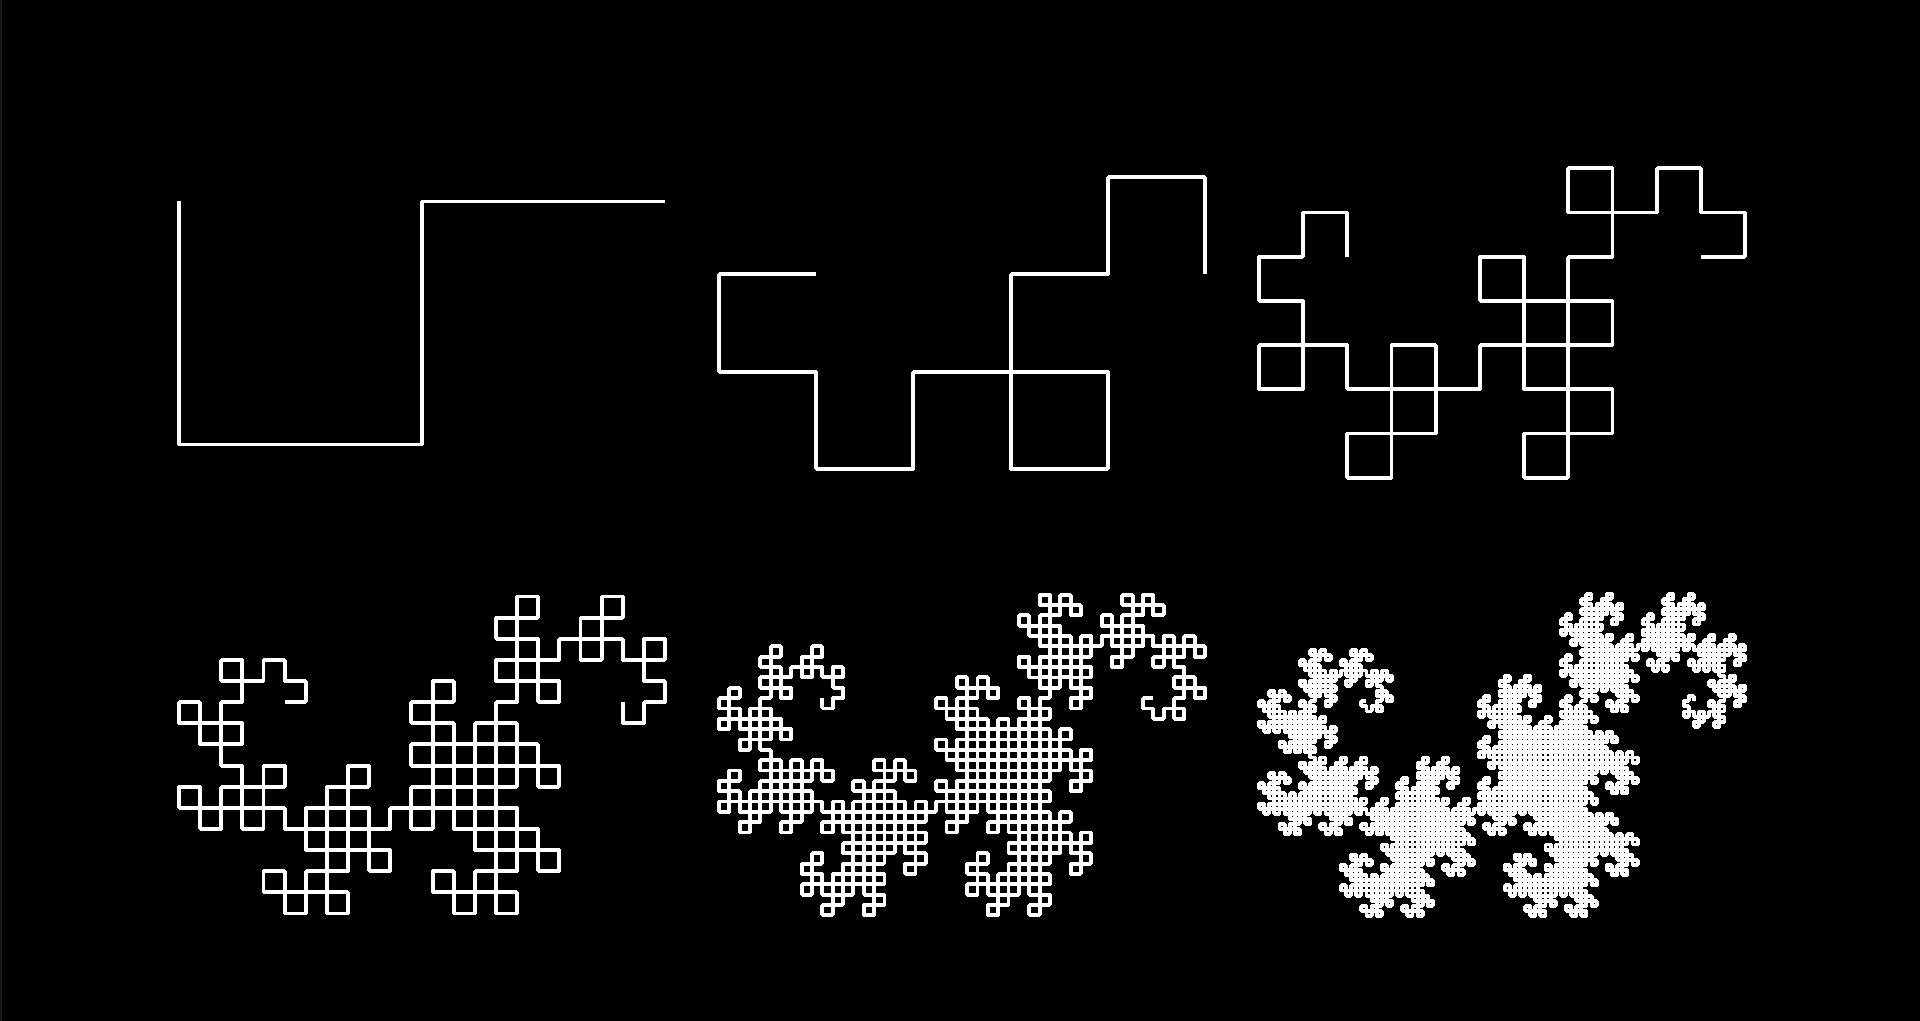
\includegraphics[width=0.66\textwidth]{Dragon Curves}
\caption{Dragon curves, generated by strings $\omega_2, \omega_4, \cdots, \omega_{12}$.}
\label{Dragon Curves}
\end{figure}

\vspace{5pt}\noindent

\subsubsection{Case Study: Runes}

Parametric L-systems \citep{hananParametricLSystems} exist as a generalisation of the above... [theory].

\vspace{5pt}\noindent
[Move into code... what parameters will we consider?]

\vspace{5pt}\noindent
[Example: various geometric runes!].

\subsubsection{Case Study: Blood Vessels} % Include post-processing!

\citet{zamirArterialBranchingLSystems} uses parametric L-systems... equations for bifurcation...

\vspace{5pt}\noindent
Suppose a branch with length $l$, width $w$ bifurcates into two branches $M$ and $m$, such that $l_M \geq l_m$. Defining the \textit{asymmetry ratio} $\alpha = l_m/l_M$, it follows that
$$l_M = \frac{l}{\left(1+\alpha^3\right)^{1/3}}, \;\; l_m = \frac{\alpha\cdot l}{\left(1+\alpha^3\right)^{1/3}}, \;\; w_M = \frac{w}{\left(1+\alpha^3\right)^{1/3}}, \;\; w_m = \frac{\alpha\cdot w}{\left(1+\alpha^3\right)^{1/3}}.$$
Furthermore, the branches diverge from their parent at angles
$$\theta_M = \arccos\left(\frac{\left(1+\alpha^3\right)^{4/3}+1-\alpha^4}{2\left(1+\alpha^3\right)^{2/3}}\right), \;\; \theta_m = \arccos\left(\frac{\left(1+\alpha^3\right)^{4/3}+\alpha^4-1}{2\alpha^2\left(1+\alpha^3\right)^{2/3}}\right).$$

\vspace{5pt}\noindent
$$\begin{matrix*}[l]
\mathbf{C} &\mapsto &\mathbf{X}[\mathbf{C}]\mathbf{C} \\
\mathbf{X} &\mapsto &\mathbf{X}\mathbf{X}
\end{matrix*}$$

\vspace{5pt}\noindent
$$\begin{matrix*}[l]
\mathbf{C} &\mapsto &\mathbf{X}[\mathbf{C}]\mathbf{C}
\end{matrix*}$$

\vspace{5pt}\noindent
$$\begin{matrix*}[l]
\mathbf{C}(l,w,\theta) &\xmapsto[0.4]{} &\mathbf{X}(l,w,\theta)[\mathbf{C}(l_M,w_M,\theta+\theta_M)]\mathbf{C}(l_m,w_m,\theta-\theta_m) \\
\mathbf{C}(l,w,\theta) &\xmapsto[0.4]{} &\mathbf{X}(l,w,\theta)[\mathbf{C}(l_m,w_m,\theta+\theta_m)]\mathbf{C}(l_M,w_M,\theta-\theta_M) \\
\mathbf{C}(l,w,\theta) &\xmapsto[0.2]{} &\mathbf{X}(l,w,\theta)\mathbf{C}(l,w,\theta) \\
\end{matrix*}$$

\vspace{5pt}\noindent
$$\begin{matrix*}[l]
\mathbf{C}(l,w,\theta) &\xmapsto[0.4]{} &\mathbf{X}(l,w,\theta)[\mathbf{L}(l_M,w_M,\theta+\theta_M)]\mathbf{R}(l_m,w_m,\theta-\theta_m) \\
\mathbf{C}(l,w,\theta) &\xmapsto[0.4]{} &\mathbf{X}(l,w,\theta)[\mathbf{L}(l_m,w_m,\theta+\theta_m)]\mathbf{R}(l_M,w_M,\theta-\theta_M) \\
\mathbf{C}(l,w,\theta) &\xmapsto[0.2]{} &\mathbf{X}(l,w,\theta)\mathbf{C}(l,w,\theta) \\
& & \\
\mathbf{L}(l,w,\theta) &\xmapsto[1.0]{} &\mathbf{X}(l,w,\theta)\mathbf{C}(l_M,w_M,\theta-\theta_M) \\
& & \\
\mathbf{R}(l,w,\theta) &\xmapsto[1.0]{} &\mathbf{X}(l,w,\theta)\mathbf{C}(l_M,w_M,\theta+\theta_M)
\end{matrix*}$$

\vspace{5pt}\noindent
\citet{liuSimulationBloodVessels} further introduce a stochastic component...


\subsection{Procedural Narrative} % TECHNIQUE: 'Improv-lite' text generation...

\section{Code Organisation}

%\subsection{HexBoard.cpp}

\subsection{Post-Processing}

\subsection{GUI}

[Include HDRR/bloom here...]

\section{Evaluation}\label{Evaluation}

\subsection{Features}

\subsection{Code Organisation}

\section{Conclusions}

\bibliographystyle{agsm}
\bibliography{../../Bibliography/Bibliography}
\addcontentsline{toc}{section}{References}
\end{flushleft}
\end{document}
